\begin{frame}
\frametitle{Aufgabe 3}
\framesubtitle{Sprungantwort des Hochpassfilters}
    \begin{figure}[H]
    \begin{center}
            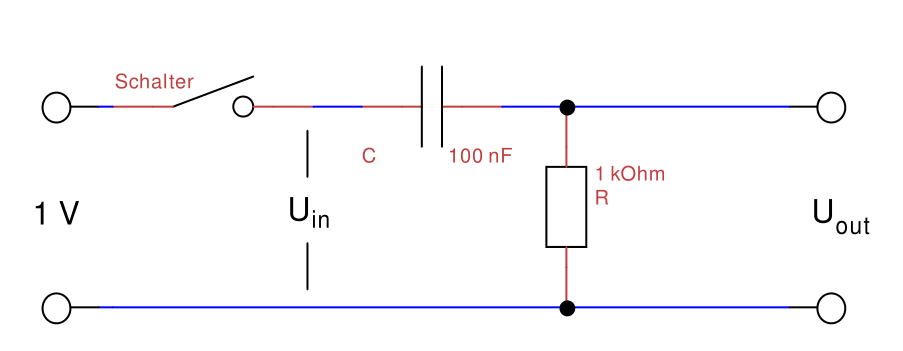
\includegraphics[scale=0.3]{./img/3_schalt.png}
    \end{center}
    \end{figure}
    
\end{frame}
\begin{frame}
    \frametitle{Aufgabe 3}
    \framesubtitle{Sprungantwort des Hochpassfilters}
     \begin{figure}[H]
     \begin{center}
             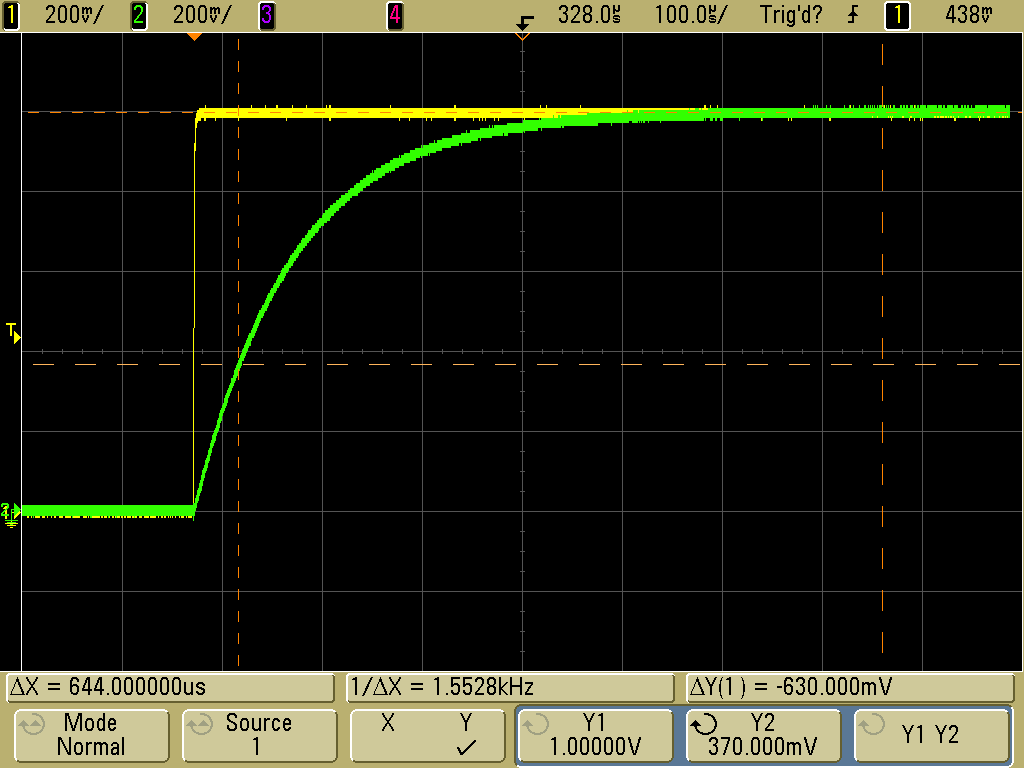
\includegraphics[scale=0.2]{./img/3_3.png}
     \end{center}
     \end{figure}
     \begin{itemize}
         \item Klassische Aufladekurve des Kondensators
         \item Charakteristische Zeit: $\tau = R \cdot C = 0.1 ms$
         \item gemessene Zeit: $\tau = - \frac{t}{\ln \left( 1-
         \frac{U(t)}{U_0}\right)} = 0.096 ms$
     \end{itemize}
\end{frame}
